\section{Outline}
\label{sec:introduction:outline}
Within this thesis, a framework for formalising model transformations will be provided, including examples and applications. In \cref{chapter:background}, more information on EMF/Ecore and GROOVE is provided. Furthermore, the theorem prover that is part of validating the proofs is introduced. In \cref{chapter:formalisations}, the formalisations of Ecore and GROOVE are introduced.
In \cref{chapter:transformation_framework}, a framework is introduced for formally expressing composable model transformations. As a part of this chapter, the formalisation of model transformations between Ecore and GROOVE is introduced. The chapter also introduces the definitions needed to compose these model transformations. \cref{chapter:library_of_transformations} introduces a non-exhaustive library of model transformations within this framework with corresponding proofs, which provides examples of the model transformations, which can be expressed within this framework. Furthermore, \cref{chapter:application} shows the composability of these model transformations by providing an example of composing smaller model transformations in a practical example. Finally, \cref{chapter:conclusion} concludes the thesis by answering the research questions and discussing possible future work.

\subsection{Mathematical notation}
\label{subsec:introduction:outline:mathematical_notation}
Throughout this thesis, a lot of mathematical definitions and proofs are introduced. In order to accommodate for these definitions and proofs, prior knowledge of commonly used mathematical notations is assumed. For completeness, the meaning of the different braces and parentheses is as follows:
\begin{itemize}
    \item Braces, ``$\{\}$'', are used to denote mathematical sets;
    \item Angle brackets, ``$\langle \rangle$'', are used to denote mathematical sequences and named tuples;
    \item Parentheses, ``$()$'', are used to denote unnamed tuples or grouping within expressions.
\end{itemize}
Besides commonly used notations, new notations are introduced as part of some definitions throughout this thesis.

\subsection{References to validated proofs}
\label{subsec:introduction:outline:references_to_validated_proofs}
As explained \cref{sec:introduction:validation}, the formal proofs within this thesis will be validated using a theorem prover. In order to easily find the validated proofs corresponding to definitions and theorems, all relevant definitions and theorems will include a reference to the validated proof. Such a reference can be recognised by the 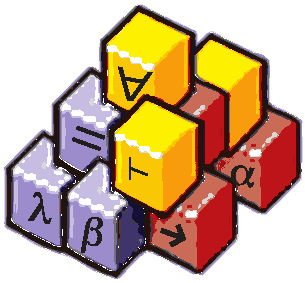
\includegraphics[height=0.75\baselineskip,keepaspectratio]{images/isabelle_logo.pdf} symbol and includes the corresponding name of the definition or theorem. For example, a reference to the theorem $mult\!\_zero\!\_unbounded\!\_valid$ from \cref{appendix:example_isabelle_theory} would be written as \isabelleref{mult_zero_unbounded_valid}{Ecore.Multiplicity}. The proofs referenced by this thesis can be found on \url{https://github.com/RemcodM/thesis-ecore-groove-formalisation}. For more information on the theorem prover used for validating the proofs within this thesis, please refer to \cref{sec:background:theorem_proving_using_isabelle}.